\section{Konzeption}
\label{sec:Konzeption}
\begin{itemize}
    \item \textbf{Proof of concept zur Machbarkeitsanalyse aus vorherigem Kapitel}
    \item \textbf{Architektur, Aufbau inkl. Diagramme etc.}
    \item \textbf{Zu entiwckelnde Komponenten auflisten und Zuständigkeiten definieren. Bspw. Doorman ist eine Referenzimplementation, die es ermöglicht auf whispers zu hören. Alternativ kann anhand von folgender Beschreibung ein eigener doorman implementiert werden...}
    \item \textbf{Schnittstellen beschreiben. bspw. Whisper für webapp<->doorman Kommunikation erwähnen, aber \emph{nicht} deb eigenen Signaturmechanismus oder den Aufbau der ausgetauschten Nachrichten}
\end{itemize}

Folgend wird das entworfene Konzept, zur Lösung der unter \ref{cha:Aufgabenstellung} beschriebenen Aufgabenstellung, beschrieben. Es umfasst den Entwurf von konkreten Systemteilen und -Komponenten, die implementiert werden müssen.

Die Webapp ermöglicht es einem Owner, ein Objekt über einen in der Blockchain festgelegten Smart Contact zu vermieten. Er kann dabei das Depot und die Mietkosten festlegen. Ein Renter kann dann dieses Objekt für eine bestimmte Zeit mieten. Die Abwicklung des Vertrages und Begleichung der Kosten geschieht über die Auslösung durch den Renter in der Blockchain. Es gibt keinen Zwischenmann (z.B. Bank), der für die Überweisung zuständig ist, sondern das Geld fliesst vom Renter direkt zum Owner, basierend auf den definierten Regeln im Smart Contract.

Abhandlung über das Fahrrad verschieben? \emph{Ein Objekt kann grundsätzlich alles sein: Ein elektrisches Fahrrad, eine Ferienwohnung oder ein Schließfach. Es muss jedoch möglich sein, einen Kontrollmechanismus anzubringen, der an eine Blockchain Node angebunden werden kann. Bei einem elektrischen Fahrrad wäre es z.B. möglich einen Minicomputer im Fahrgestellt zu montieren, welcher den Akku aktiviert oder deaktiviert und über eine Sim-Karte mit der Blockchain synchronisiert. Möchte ein Benutzer das Fahrrad verwenden, so müsste er dieses zuerst über die Blockchain mieten und erst dann kann er den Akku aktivieren. Die Mietkosten würden über den Smart Contract dem Anbieter des Fahrrades überwiesen werden.}

\begin{figure}
\centering
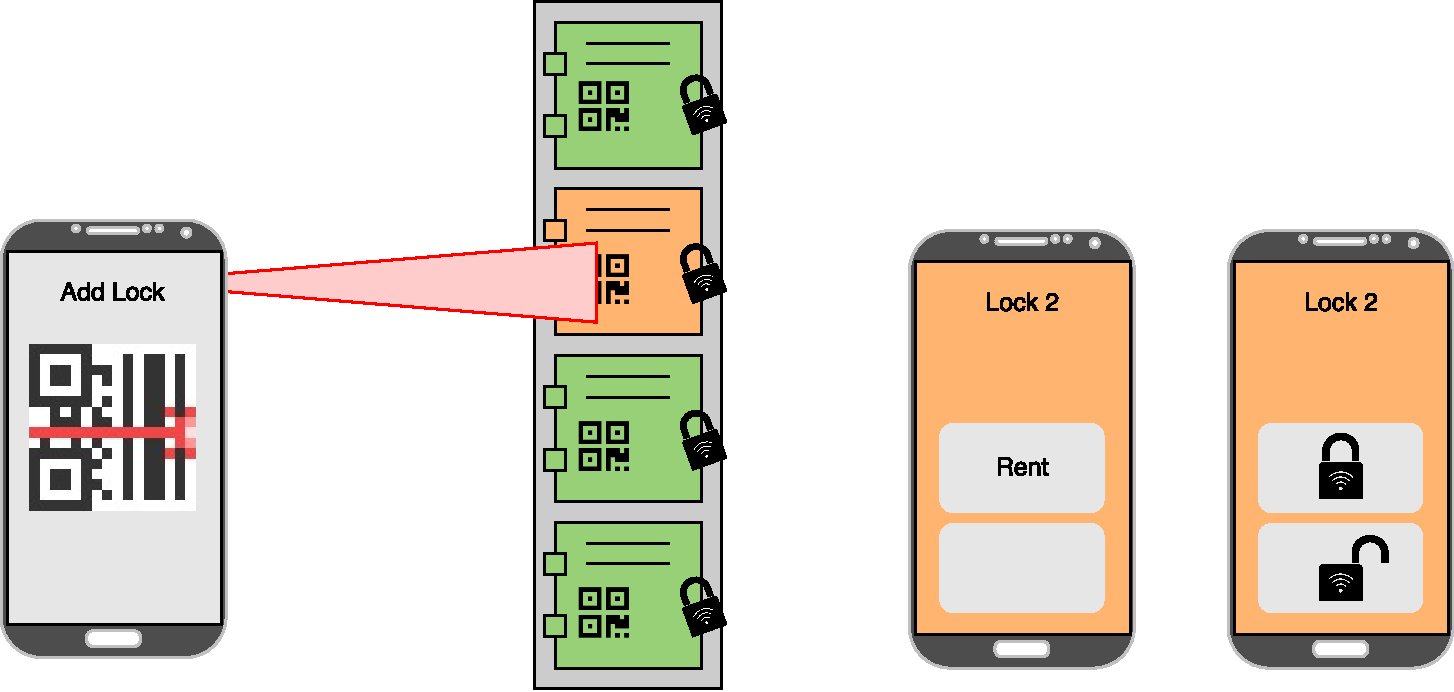
\includegraphics[width=.95\textwidth]{Mobile_Konzept}
\caption{Das Mobile-Konzept, dessen Umsetzung möglich ist}
\label{fig:Mobile_Konzept}
\end{figure}

\subsection{Interaktion mit dem Demonstrator}
\label{sec:Interaktion mit dem Demonstrator}

Ein Benutzer muss sich zuerst als einen weiteren Node mit der Blockchain verbinden. Anschliessend kann er über die entwickelte Webapp (DAPP) mit dem System interagieren. 

\vspace{1em}\noindent
Folgende Interaktionen sind möglich.

\vspace{1em}\noindent
\textbf{Als Owner}
\begin{itemize}
    \item Neues Rentable (Objekt) erfassen
    \item Bestehende Rentable deaktivieren/aktivieren/zerstören
\end{itemize}

\vspace{1em}\noindent
\textbf{Als Renter}
\begin{itemize}
    \item Neues Rentable eintragen
    \item Informationen und Verfügbarkeit eines Rentables prüfen
    \item Ein Rentable reservieren (rent)
\end{itemize}

\vspace{1em}\noindent
\textbf{Als aktueller Renter (current renter)}
\begin{itemize}
    \item Sperren und Entsperren des Rentables (Lock/Unlock)
    \item Zurückgeben des Schließfachs (Unclaim)
\end{itemize}

\subsection{Regeln}
\begin{enumerate}
    \item Hat zum aktuellen Zeitpunkt niemand das Rentable reserviert, so ist der Owner gleich dem Renter.
    \item Es gibt keine Reservationsüberlappungen
    \item Eine aktive Reservation kann mittels \emph{Emergency} verlängert werden. Steht die Verlängerung im Konflikt mit einer nächsten Reservation, so wird der Startzeitpunkt der Reservation nach hinten verschoben. Wird im Fallbeispiel ... erläutert.
    \item ...
\end{enumerate}

\subsection{Fallbeispiele}
\label{sec:Fallbeispiele}
Die folgenden Fallbeispiele erläutern das Zusammenspiel der Interaktionen und die Verschiebung der priviligierten Rechte entlang der Zeitachse.

\subsubsection{Normal-Fall}
In Abb.~\ref{fig:Cases}\,(a) reserviert Benutzer A das Schliessfach von $t_{R1}$ bis $t_{R2}$ zum Zeitpunkt $t_0$. Das Deposit und die Mietkosten werden ihm somit abgezogen.
Zum Zeitpunt $t_{R1}$ wird Benutzer A zum \emph{Current Renter} und besitzt dadurch privilegierten Zugriff. Er kann jetzt das Schliessfach öffnen (Unlock) und schliessen (Lock). Nach einer gewissen Zeit noch vor Ablauf der Reservation, entschliesst sich Benutzer A das Schliessfach wieder abzugeben (Unclaim), da er es nicht mehr benötigt. Die Reservation wird somit auf diesen Zeitpunkt gekürzt und Benutzer A erhählt sein Deposit und die Mietkosten für die ungenutzte Zeit zurück. Die priviligierten Rechte werden umgehend wieder an den Owner abgegeben.

\begin{figure}
\centering\small
\setlength{\tabcolsep}{0mm}	% alle Spaltenränder auf 0mm
\begin{tabular}{c@{\hspace{12mm}}c} % mittlerer Abstand = 12mm
  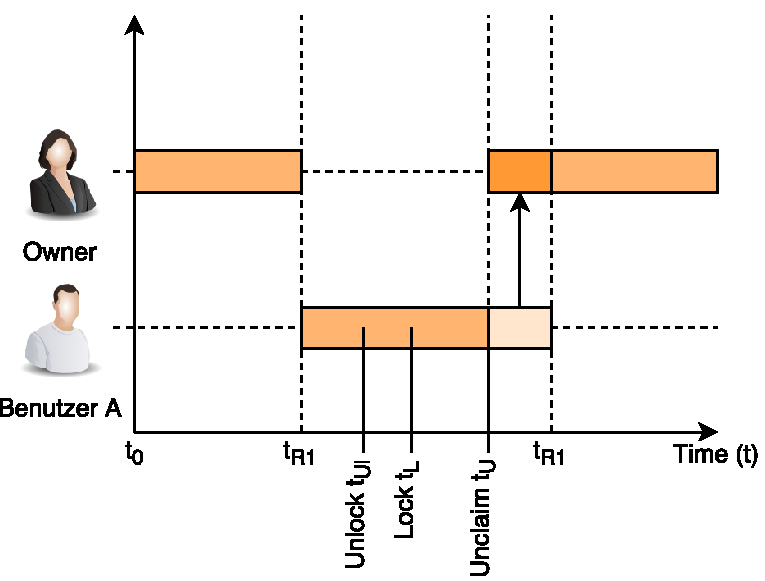
\includegraphics[width=.45\textwidth]{Case-Normal} &
  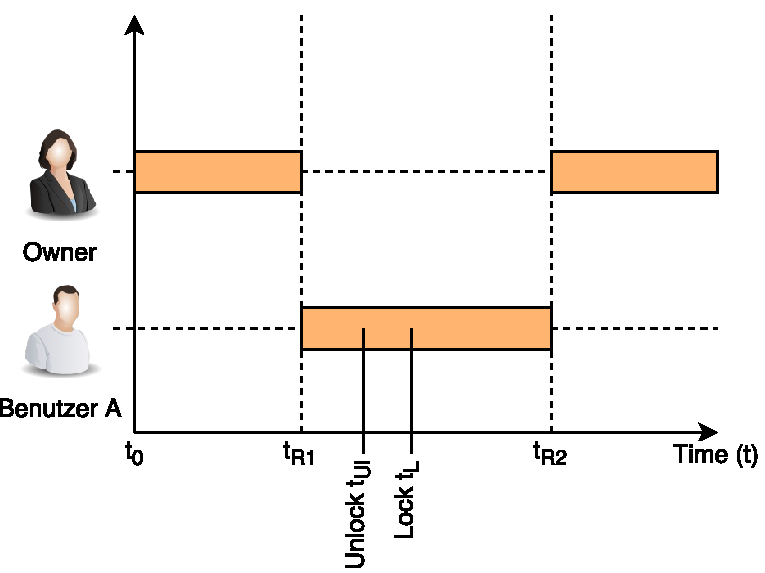
\includegraphics[width=.45\textwidth]{Case-No-Unclaim} \\
  (a) & (b)
  \\[1em]	%vertical extra spacing (4 points)
  \multicolumn{2}{c}{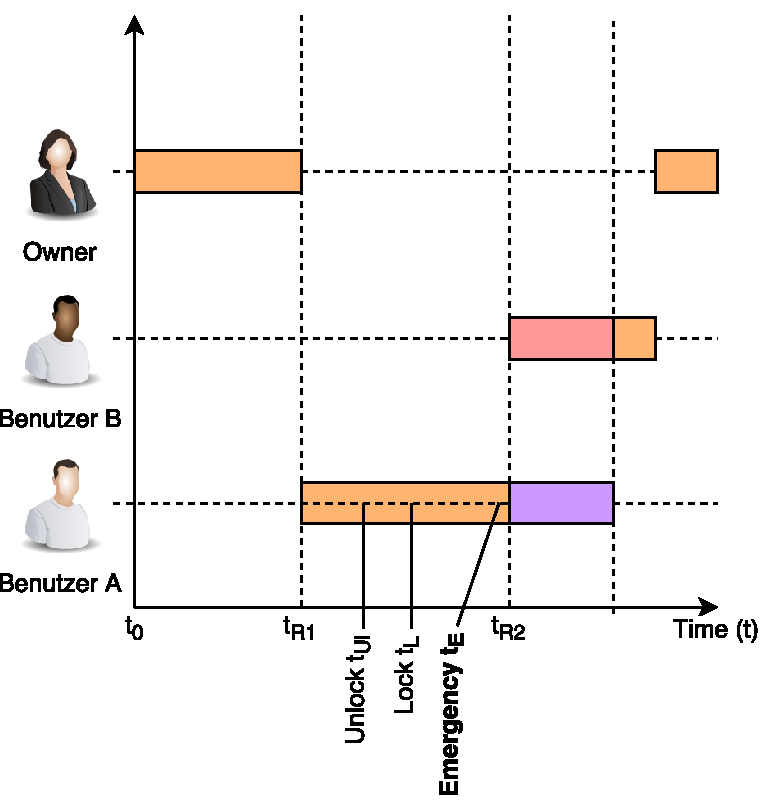
\includegraphics[width=.45\textwidth]{Case-Emergency}}\\
  \multicolumn{2}{c}{(c)} 
\end{tabular}
%
\caption{Verschiedene Fälle -- 
Normal-Fall (a), Keine-Rückgabe (b),
Emergency-Fall (c).}
\label{fig:Cases}
\end{figure}

%\begin{figure}
%\centering
%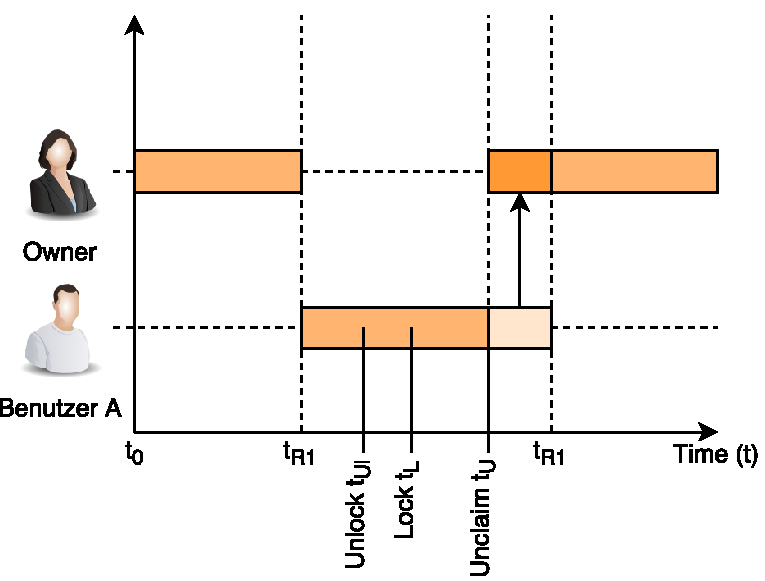
\includegraphics[width=.95\textwidth]{Case-Normal}
%\caption{Normal-Fall}
%\label{fig:Case-Normal}
%\end{figure}

\subsubsection{Reservationsende ohne Betätigung der Rückgabe}
Wie im Normal-Fall beschrieben, ist Benutzer A momentaner Renter (current renter) des Schliessfaches. Anstelle jedoch das Schließfach wieder zurückzugeben, lässt er die Reservationszeit auslaufen. Zum Zeitpunkt $t_{R2}$ werden ihm die Rechte entzogen und er erhält keine Rückerstattung des Deposits. Es liegt also in Benutzer A seinem Interesse, alle eingeschlossenen Gegestände vor Ablauf der Reservation aus dem Schließfach zu nehmen und dieses zurückzugeben (Unclaim). Siehe Abb.~\ref{fig:Cases}\,(b) als Illustration.

\subsubsection{Emergency zum Verlängern der Reservationsdauer}
Der Benutzer A sollte immer einen Buffer in die Reservationszeit einplanen, damit er das Schließfach auch noch bei Zugsausfall oder einem Autounfall rechtzeitig vor Reservationsablauf erreichen kann. In äußersten Notfällen kann es trotzdem vorkommen, dass der Benutzer A nicht rechtzeitig seine Affären aus dem Schließfach nehmen kann und aus diesem Grund hat er die Möglichkeit eine \emph{Emergency} auszulösen. Die Emergency ist entsprechend kostenintensiv und sollte deswegen nur in Notfällen und abhängig vom Wert der Gegenstände im Schließfach in Erwägung gezogen werden. 
Die Emergency verhindert den Ablauf der aktuellen Reservation und überschreibt allenfalls nachfolgende Reservationen. Betroffene Reservationen erhalten einen Teil der Einnahmen durch die Emergency als Entschädigung. Die Abbildung \ref{fig:Cases}\,(c) veranschaulicht dieses Scenario.

\subsubsection{Fall von Schäden}
Benutzer A reserviert wie im Normal-fall ein Schliessfach. Zum Zeitpunkt t1 will er das Schliessfach öffen (Unlock), dieses reagiert jedoch nicht. Er muss nun Kontakt mit dem Owner aufnehmen und die Sache klären. Auf jeden Fall sollte er nun das Schliessfach zurückgeben (Unclaim) um die Kosten niedrig zu halten, im Falle, dass sich der Owner nicht auffinden lässt oder dieser kein Interesse zeigt.

Im Rahmen dieser Arbeit wurde auch ein Konzept überlegt, wie solche Probleme vermindert werden könnten. Durch Einführen eines Review Systems, wo Benutzer die Owner beurteilen können. Owner mit einer guten Bewertung (Score) wären dann vertrauenswürdiger.

\begin{itemize}
    \item \textbf{ Wie funktioniert unsre Loesung? }
    \item \textbf{ Was ermoeglicht unsere Loesung? }
    \item \textbf{ Wie sicher ist das System? }
    \item \textbf{ Was sind moegliche Angriffe? }
    \item \textbf{ Wie stehts mit der Verfuegbarkeit?}
    \item \textbf{ Gibt es Restrictions?}
    \item \textbf{ Was sind die Staerken und Schwaechen dieser Loesung? }
    \item \textbf{ Wie ist der Ablauf? Was geschieht wann?\ref{sec:Fallbeispiele}}
    \item \textbf{ Was kann der Benutzer machen? \ref{sec:Interaktion mit dem Demonstrator}}
    \item \textbf{ Wie sind die Regeln? Wer kann reservieren und wann? Was passiert, wenn die Reservation ablauft? Wer haftet? Was ist, wenn das Schliessfach beschaedigt ist und ich es nicht antreten kann?\ref{sec:Fallbeispiele}}
    \item \textbf{ Wie sieht das Kostenmodel aus? Beispiele und Scenarien?}
    \item \textbf{ Wer nutzt unsere Loesung? }
    \item \textbf{ Warum nutzt man unsere Loesung?}
    \item \textbf{ Was sind Scenarien, wo unsere Loesung zum einsatz kommen wuerde?}
    \item \textbf{ Wie ist der grobe Aufbau?}
    \item \textbf{ Was fuer Technologien setzen wir ein und weshalb Blockchain?}
    \item \textbf{ Wie ist die Interaktion mit dem Benutzer? Kontextdiagramm? Es gibt mehrere Benutzer und Rollen.}
    \item \textbf{ Was brauchts um diese Loesung um zu setzten? Smart Contracts, Blockchain, Hardware, WebUI }
    \item \textbf{ In welche Komponenten ist das System aufgeteilt. Was sind die eizelnen Funktionen?}
    \item \textbf{ Was sind die Abhaengikeiten unseres Systems?}
    \item \textbf{ Wie sehen die Schnittstellen aus?} 
    \item \textbf{ Was fuer Technologien werden eingesetzt?} 
    \item \textbf{ Wie sieht das Design der Komponenten aus? Erweiterbar? Wartbar?} 
    \item \textbf{ Wie sieht das User Interface aus?} 
    \item \textbf{ Welche Libraries verwenden wir? Was haben wir entwickelt?}
    \item \textbf{ Wie wird das System deployed?}
    \item \textbf{ Kann man updates fahren?}
    \item \textbf{ Schrittanleitung zur Installation?}
\end{itemize}

\subsection{Nutzen von Blockchain}
Warum ist blockchain besser als "server unten rein stellen"?
